\documentclass{article}
\usepackage[utf8]{inputenc}
\usepackage[english,russian]{babel}
\usepackage{graphics}
\usepackage{amsmath}
\usepackage{graphicx}
\graphicspath{{./pic/}}
\usepackage[pdftex]{graphicx}

\begin{document}
\graphicspath{{trash from tex/}}
\DeclareGraphicsExtensions{.pdf,.png,.jpg}
\begin{document}
	1.Задание 23 №311923
\par
\par
постройте график функции
 $
\begin{cases}
-x^2-4x-4&\text{,если $x<-1$,}\\
1-|x-1| &\text{,если$x\geqslant-1$,}
\end{cases}
$
\par
и определите, при каких значениях параметра {$a$} он имеет ровно две общие точки с прямой {$y=a$}
\par
Решение
\par
построим график этой функции:
\par
\begin{figure}[h]
	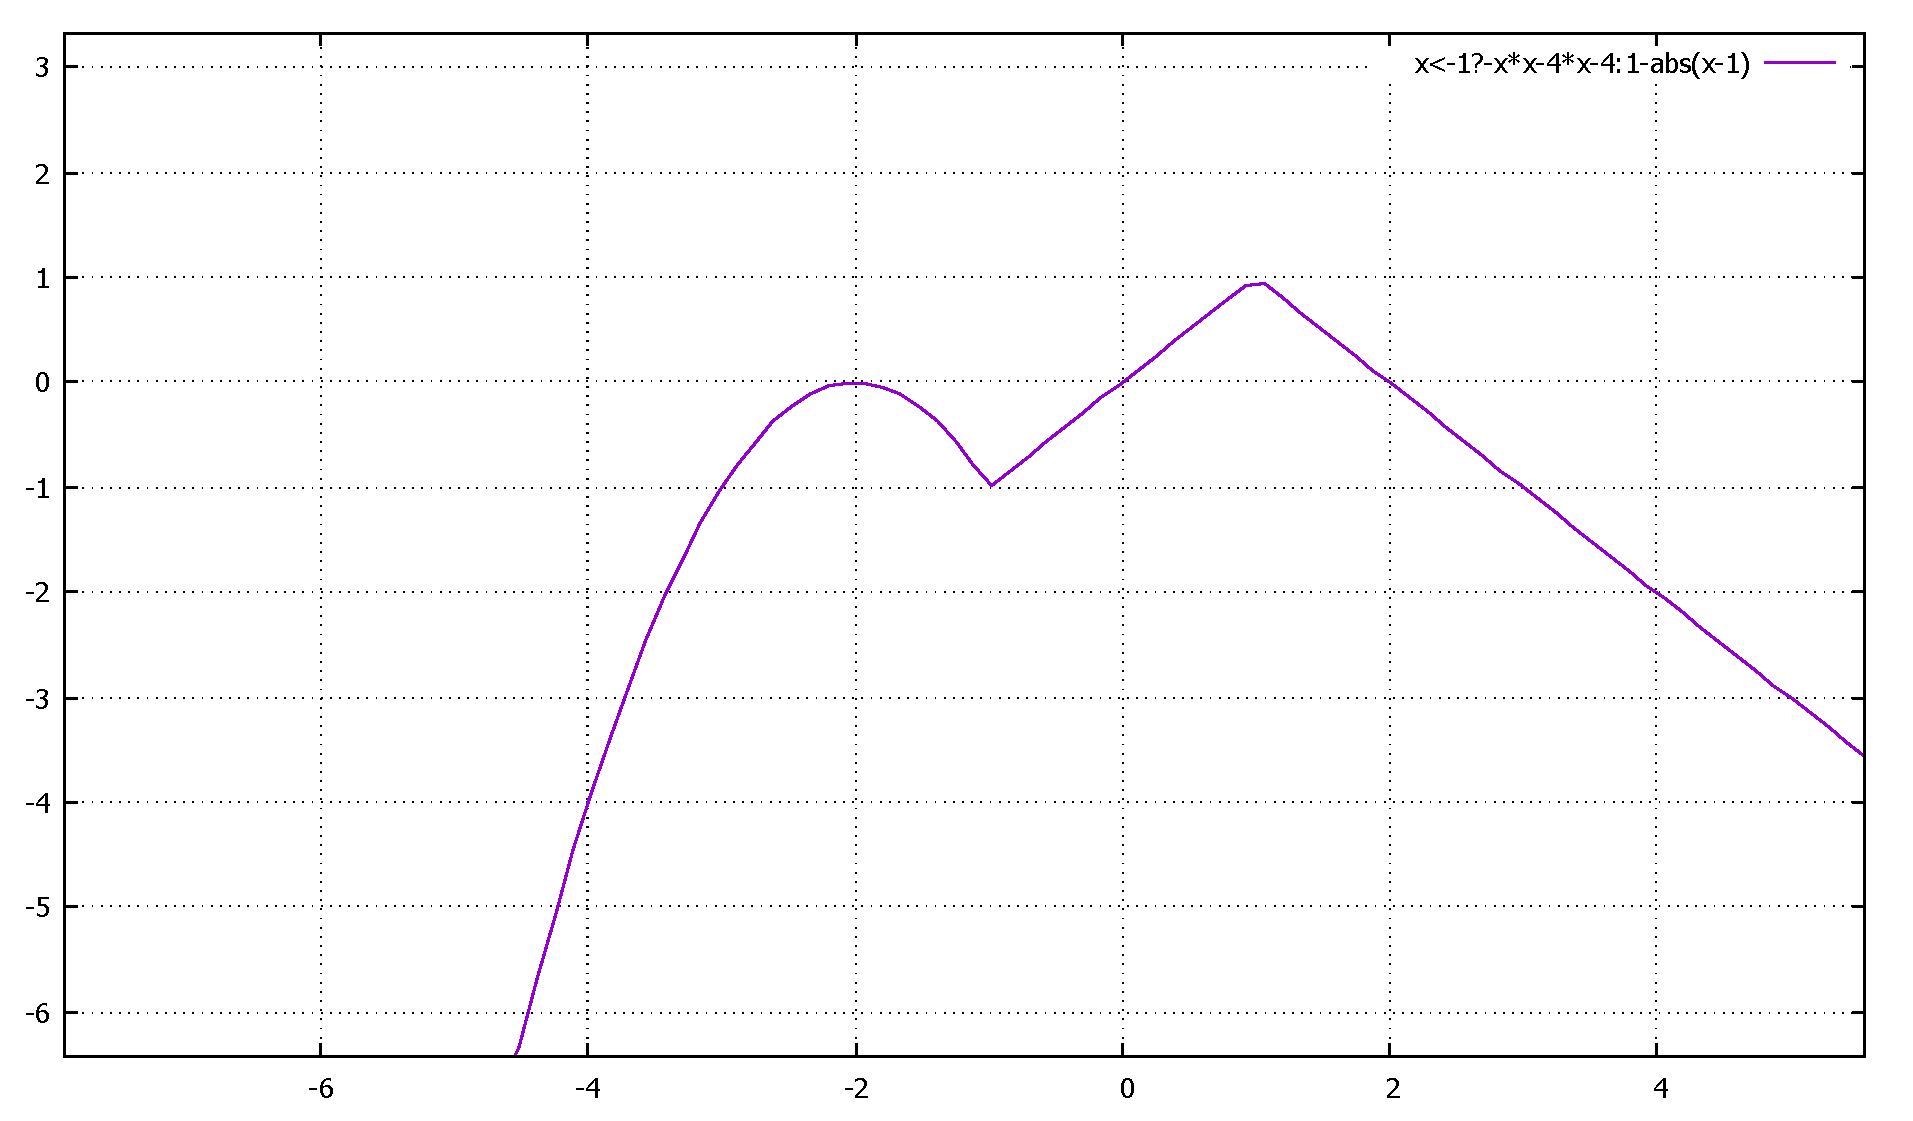
\includegraphics[scale=0.5]{superplot.pdf}
	\caption{График}
	\label{fig:image}
\end{figure}
\par
Исходя из вышеприведенного графика можно сделать вывод, что: 
\par
{$a\in(-\infty;-1)\bigcup(0;1) $}
\end{document}
\end{document}
